% Options for packages loaded elsewhere
\PassOptionsToPackage{unicode}{hyperref}
\PassOptionsToPackage{hyphens}{url}
\PassOptionsToPackage{dvipsnames,svgnames,x11names}{xcolor}
%
\documentclass[
  openany]{book}
\usepackage{amsmath,amssymb}
\usepackage{lmodern}
\usepackage{iftex}
\ifPDFTeX
  \usepackage[T1]{fontenc}
  \usepackage[utf8]{inputenc}
  \usepackage{textcomp} % provide euro and other symbols
\else % if luatex or xetex
  \usepackage{unicode-math}
  \defaultfontfeatures{Scale=MatchLowercase}
  \defaultfontfeatures[\rmfamily]{Ligatures=TeX,Scale=1}
\fi
% Use upquote if available, for straight quotes in verbatim environments
\IfFileExists{upquote.sty}{\usepackage{upquote}}{}
\IfFileExists{microtype.sty}{% use microtype if available
  \usepackage[]{microtype}
  \UseMicrotypeSet[protrusion]{basicmath} % disable protrusion for tt fonts
}{}
\makeatletter
\@ifundefined{KOMAClassName}{% if non-KOMA class
  \IfFileExists{parskip.sty}{%
    \usepackage{parskip}
  }{% else
    \setlength{\parindent}{0pt}
    \setlength{\parskip}{6pt plus 2pt minus 1pt}}
}{% if KOMA class
  \KOMAoptions{parskip=half}}
\makeatother
\usepackage{xcolor}
\IfFileExists{xurl.sty}{\usepackage{xurl}}{} % add URL line breaks if available
\IfFileExists{bookmark.sty}{\usepackage{bookmark}}{\usepackage{hyperref}}
\hypersetup{
  pdftitle={    PhD Handbook   2022-2023 Academic Year },
  pdfauthor={PhD Program Leadership},
  colorlinks=true,
  linkcolor={Maroon},
  filecolor={Maroon},
  citecolor={Blue},
  urlcolor={blue},
  pdfcreator={LaTeX via pandoc}}
\urlstyle{same} % disable monospaced font for URLs
\usepackage{longtable,booktabs,array}
\usepackage{calc} % for calculating minipage widths
% Correct order of tables after \paragraph or \subparagraph
\usepackage{etoolbox}
\makeatletter
\patchcmd\longtable{\par}{\if@noskipsec\mbox{}\fi\par}{}{}
\makeatother
% Allow footnotes in longtable head/foot
\IfFileExists{footnotehyper.sty}{\usepackage{footnotehyper}}{\usepackage{footnote}}
\makesavenoteenv{longtable}
\usepackage{graphicx}
\makeatletter
\def\maxwidth{\ifdim\Gin@nat@width>\linewidth\linewidth\else\Gin@nat@width\fi}
\def\maxheight{\ifdim\Gin@nat@height>\textheight\textheight\else\Gin@nat@height\fi}
\makeatother
% Scale images if necessary, so that they will not overflow the page
% margins by default, and it is still possible to overwrite the defaults
% using explicit options in \includegraphics[width, height, ...]{}
\setkeys{Gin}{width=\maxwidth,height=\maxheight,keepaspectratio}
% Set default figure placement to htbp
\makeatletter
\def\fps@figure{htbp}
\makeatother
\setlength{\emergencystretch}{3em} % prevent overfull lines
\providecommand{\tightlist}{%
  \setlength{\itemsep}{0pt}\setlength{\parskip}{0pt}}
\setcounter{secnumdepth}{5}
% margins
\usepackage[left=3.175cm,right=3.175cm,top=3.175cm,bottom=3.175cm]{geometry}

% sections in sans serif
\usepackage{sectsty}
\chapterfont{\large\bfseries}
\sectionfont{\large\bfseries}
\subsectionfont{\large\bfseries}
\allsectionsfont{\sffamily}

\usepackage{fontsize}
  \changefontsize[12.8pt]{12pt}

% avoid figure on its own page
\renewcommand{\floatpagefraction}{.8}

% no paragraph indentation
\setlength\parindent{0pt} 
\usepackage{booktabs}
\usepackage{longtable}
\usepackage{array}
\usepackage{multirow}
\usepackage{wrapfig}
\usepackage{float}
\usepackage{colortbl}
\usepackage{pdflscape}
\usepackage{tabu}
\usepackage{threeparttable}
\usepackage{threeparttablex}
\usepackage[normalem]{ulem}
\usepackage{makecell}
\usepackage{xcolor}
\ifLuaTeX
  \usepackage{selnolig}  % disable illegal ligatures
\fi
\usepackage[]{natbib}
\bibliographystyle{apalike}

\title{
\includegraphics[width=6.25in,height=\textheight]{mcgill-epi-logo.png} PhD Handbook 2022-2023 Academic Year}
\author{PhD Program Leadership}
\date{2022-08-25}

\begin{document}
\maketitle

{
\hypersetup{linkcolor=}
\setcounter{tocdepth}{1}
\tableofcontents
}
\hypertarget{preface}{%
\chapter*{Preface}\label{preface}}
\addcontentsline{toc}{chapter}{Preface}

Note that this handbook is specific to the Epidemiology program and does not replace McGill's Graduate and Postdoctoral Studies (GPS) \href{https://www.mcgill.ca/students/courses/calendars/}{Calendar} or \href{https://www.mcgill.ca/gps/students/policies-and-guidelines}{Policies and Procedures}. You are responsible for reading and understanding the official GPS procedures, rules and regulations. Please contact the Epidemiology Graduate Program Director (GPD) or Student Services Office to answer any questions.

\hypertarget{introduction}{%
\chapter{Introduction}\label{introduction}}

Welcome to the the PhD program in Epidemiology at McGill. This handbook aims to provide an overview of important requirements for completing your degree, as well as providing links to other sources of information to enhance your experience in the program.

Epidemiology is the study and analysis of the patterns and causes of disease in human populations. It forms the core discipline of public health by identifying the distribution and determinants of health and disease, and by gaining the etiologic understanding to intervene toward the improvement of population health. The PhD program in epidemiology at McGill trains scientists and health professionals to design and conduct studies, analyze health data and effectively communicate scientific results, and to gain novel insights into the causes and prevention of diseases at the population level. Epidemiologic work at the doctoral level involves a thorough integration of biological knowledge of pathogenesis, statistical knowledge of quantitative analysis and causal inference, and sociological knowledge to place these insights in the context of dynamic and interconnected human populations. Major areas of strength at McGill include epidemiologic methods, clinical epidemiology, infectious diseases, social epidemiology, pharmacoepidemiology, public and population health, global health, environmental epidemiology, chronic diseases and aging, and perinatal epidemiology.

\hypertarget{phd-program-leadership}{%
\section{PhD Program Leadership}\label{phd-program-leadership}}

\emph{Program Director}\\
Sam Harper (\href{mailto:sam.harper@mcgill.ca}{\nolinkurl{sam.harper@mcgill.ca}})\\
Phone: 514-398-2356\\
Office: 2001 McGill College, Suite 1262

\emph{Program Advisor}\\
Kris Filion (\href{mailto:kristian.filion@mcgill.ca}{\nolinkurl{kristian.filion@mcgill.ca}})\\
Phone: 514-340-8222 x 28394\\
Office: Centre for Clinical Epidemiology, Jewish General Hospital (Lady Davis Institute)

\emph{Student Affairs Officer}\\
André Yves Gagnon (\href{mailto:gradadmin.eboh@mcgill.ca}{\nolinkurl{gradadmin.eboh@mcgill.ca}})\\
Phone: 514-398-1812\\
Office: 2001 McGill College, Suite 1253

\emph{Administrative Student Affairs Coordinator}\\
Katherine Hayden (\href{mailto:gradcoord2.eboh@mcgill.ca}{\nolinkurl{gradcoord2.eboh@mcgill.ca}})\\
Phone: 514-398-6269\\
Office: 2001 McGill College, Suite 1250

\emph{PhD Student Representative}\\
Leah Flatman (\href{mailto:leah.flatman@mail.mcgill.ca}{\nolinkurl{leah.flatman@mail.mcgill.ca}})

\hypertarget{competencies}{%
\section{Competencies}\label{competencies}}

Our program aims to prepare our students for successful careers in epidemiology. Upon successful completion of the PhD in Epidemiology at McGill, we aim for our students to:

\begin{itemize}
\tightlist
\item
  Understand the difference between descriptive, predictive, and etiologic epidemiologic studies, and the value of different study designs for epidemiologic science;
\item
  Develop a thorough understanding of modern epidemiologic methods and how they are utilized in the service of answering epidemiologic questions;
\item
  Apply quantitative skills to the analysis of epidemiologic data using statistical software;
\item
  Systematically and critically review the epidemiologic literature, synthesize existing evidence, and identify important gaps in knowledge;
\item
  Design, write, and critique an independent research proposal for answering epidemiologic questions;
\item
  Develop skills in communicating epidemiologic findings to a variety of audiences (professional, student, lay) and through a variety of formats, including oral and written reports.
\end{itemize}

\hypertarget{high-level-program-overview}{%
\section{High-Level Program Overview}\label{high-level-program-overview}}

Successful completion of the PhD program in EBOH involves 4 key milestones:\\
- Required coursework;\\
- Passing a comprehensive exam;\\
- Developing and defending a thesis protocol; and\\
- Writing and defending the doctoral thesis.

The timeline for program completion varies depending on each student's circumstances and subject matter, but most of our students complete the PhD in around 5 years.

\hypertarget{example-timeline-and-milestones}{%
\section{Example Timeline and Milestones}\label{example-timeline-and-milestones}}

Below we show a very general example of a timeline for completing all of the required coursework and other milestones, as well as some reporting requirements.

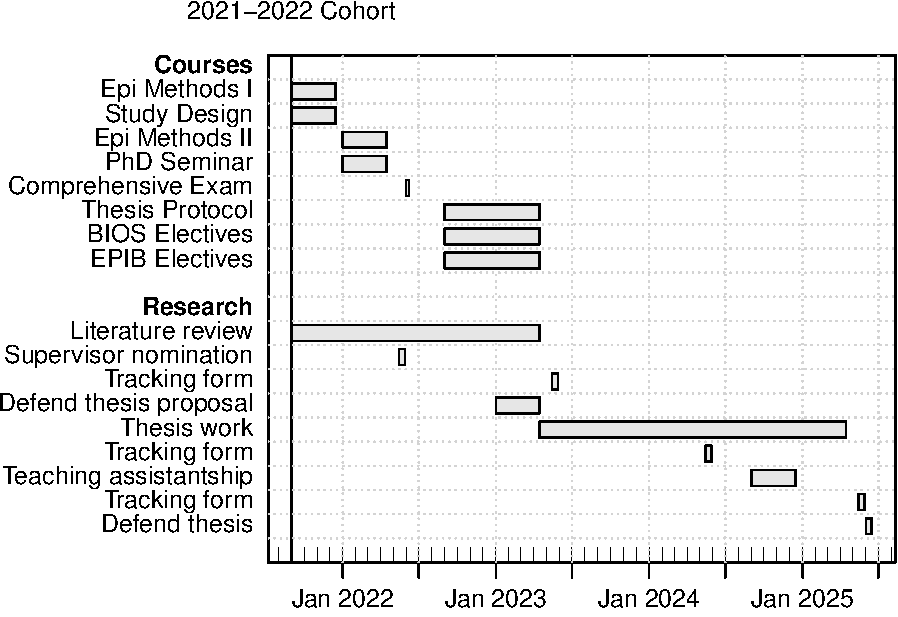
\includegraphics{01-Introduction_files/figure-latex/plan-1.pdf}

\hypertarget{supervision}{%
\chapter{Supervision}\label{supervision}}

Supervision plays a crucial role in your doctoral training, so the decision of choosing a supervisor should be made with care and attention. Consider your substantive research interests, funding, timelines, how much time and responsiveness you may need from a supervisor, as well as a potential supervisor's existing supervision load when making your decision. Don't be afraid to ask lots of questions about a supervisor's style of working or research group policies before committing to work with someone.

\hypertarget{getting-started}{%
\section{Getting Started}\label{getting-started}}

By default, all doctoral students, even those that have previously discussed supervision with a faculty member, are initially advised by the designated PhD Program Advisor. The advisor's role is to provide early guidance on your academic program and career planning, to mentor you, and to serve as your advocate when necessary. Generally speaking, once a supervisor has been approved, the supervisor takes on the primary mentorship role.

Of course, this does not exclude the possibility of a student-supervisor match at admission, nor the possibility of the academic Program Advisor becoming a student's supervisor.

\hypertarget{thesis-supervisor}{%
\section{Thesis Supervisor}\label{thesis-supervisor}}

Doctoral students are expected to identify a supervisor by no later than 15 February of their first year of study, but identifying a supervisor earlier is encouraged, as solid supervision is important for planning and making progress.

If you currently don't have a supervisor, take the time to contact professors within the various areas of faculty research that interest you. Faculty research interests are broadly categorized on the departmental \href{https://www.mcgill.ca/epi-biostat-occh/research}{website}. It is also worthwhile networking and discussing potential supervisors with your peers and more senior doctoral students. If you wish to be supervised by an \href{https://www.mcgill.ca/epi-biostat-occh/people/field_mprofile_group/Associate\%20Members}{Associate Member} of the department it may be necessary to have a Full Member of the faculty as a co-supervisor. Contact the Student Services Office or the Program Director/Advisor for assistance.

Although uncommon, note that it is certainly possible to change thesis supervisors at any point during your training. Generally, if you plan to change supervisors, it is advantageous to do so earlier rather than later in your training. Changing supervisors has consequences for funding and possibly your thesis topic and timeline, and should be carefully considered. Before you make a decision to change, talk to the PhD program administrators.

\hypertarget{requirements}{%
\section{Requirements}\label{requirements}}

Your thesis supervisor must be a McGill faculty member with an appointment in the Department of Epidemiology, Biostatistics and Occupational Health. In the course of formalizing your decision on a supervisor, note that both students and supervisors are required to sign a Letter Of Understanding. This document is designed to promote dialogue between the supervisor(s) and the graduate student to define their expectations and to increase awareness of the rights and responsibilities governing the training program and the student-supervisor relationship. The aim is to avoid problems and to achieve a positive and mutually beneficial experience. It is due at the same time as the Thesis Supervisor Nomination form, May 15 at the end of the first year. The Supervisor Nomination Form and the Letter of Understanding are available \href{https://www.mcgill.ca/epi-biostat-occh/files/epi-biostat-occh/eboh_supervisor_nomination_form-lou_201909.docx}{here}.

\hypertarget{suggestions}{%
\section{Suggestions}\label{suggestions}}

Maintaining a mutually respectful and supportive relationship with your thesis supervisor will help make your journey through the program easier. To ensure timely progress through the degree program, we recommend discussing the following issues with your supervisor at the earliest opportunity after admission. Any unresolved issues should be reviewed periodically and agreement achieved as soon as possible. It might be helpful to attach to this checklist detailed minutes of discussions held and decisions made, as appropriate.

\textbf{Issues to Discuss:}

\begin{itemize}
\tightlist
\item
  Course plan: courses; credits by semester
\item
  Thesis timeline: dates for protocol; completion
\item
  Thesis format: classic or manuscript based
\item
  Authorship: number of expected papers; content, journals; first, senior, co-authors, corresponding author; number of presentations, content, conference locations, costs
\item
  Thesis project: possible topics; primary or secondary data collection; holding rights \& responsibilities
\item
  Members of supervisory committee: proposed; confirmed
\item
  Committee meetings: number and timing; by semester
\item
  Funding: personal, project
\item
  Ethics approval: timing
\item
  Office hours: hours, open door
\item
  Absences: sabbatical; holidays; conferences
\end{itemize}

\hypertarget{thesis-supervisory-committee}{%
\section{Thesis supervisory committee}\label{thesis-supervisory-committee}}

You are required to have a Thesis Supervisory Committee. The membership and size are determined by you and your supervisor, with the approval of the PhD Program Director or Advisor. For the PhD a minimum committee of two (your supervisor and one other member) is required, but may (and likely should) be larger, depending on how inter-disciplinary the topic is, and what other expertise is needed to support your thesis. Committee members must hold a faculty or scientist appointment at a university or research institution, though there is flexibility to include members at non-research institutions if needed. The committee should be struck at an early stage of thesis research and certainly no later than the end of the semester in which the topic has been defined.

Meetings with the entire thesis supervisory committee should be held as frequently as is necessary to ensure efficient progress of the thesis research, but at a \emph{minimum} once per semester.

\hypertarget{expectations}{%
\section{Expectations}\label{expectations}}

\hypertarget{expectations-for-the-supervisor}{%
\subsection{Expectations for the supervisor}\label{expectations-for-the-supervisor}}

A Supervisor will:

\begin{itemize}
\tightlist
\item
  help to define topic of dissertation;
\item
  help to assemble Supervisory Committee;
\item
  jointly with you, notify department in writing of topic and committee members;
\item
  help to define exact nature and scope of dissertation;
\item
  meet, or otherwise communicate, with you at least once a month;
\item
  provide timely feedback;
\item
  monitor deadlines;
\item
  be aware of, and coordinate (and resolve any conflicts in) any advice received by you when you meeting separately with other members of Supervisory Committee or with other consultants
\item
  hold once-a-semester meeting of full Supervisory Committee;
\item
  when thesis is nearing completion, submit names of possible examiners to Department;
\item
  ensure that corrections/suggestions by examiners are carried out.
\end{itemize}

\hypertarget{expectations-for-thesis-committee-members}{%
\subsection{Expectations for Thesis Committee Members}\label{expectations-for-thesis-committee-members}}

Thesis Committee Members will:

\begin{itemize}
\tightlist
\item
  be a consultant to you and your supervisor;
\item
  evaluate (with other members of thesis committee) and when satisfied, formally approve your research protocol;
\item
  attend once-a-semester meeting of your full thesis committee and take active part in assessing progress and setting goals for you.
\end{itemize}

\hypertarget{expectations-for-you}{%
\subsection{Expectations for you}\label{expectations-for-you}}

The department expects that you will:

\begin{itemize}
\tightlist
\item
  follow the timelines set out for the program, including submitting the required progress reports in accordance with established deadlines;
\item
  establish a thesis committee, and convene meetings of this committee on a regular basis, ensuring there is at least one full committee meeting per semester;
\item
  be a full-time research student, and keep research moving forward in accordance with the timetable for completion of activities noted in the annual work plan you are to submit;
\item
  follow established norms for research integrity.
\end{itemize}

\hypertarget{conflicts}{%
\section{Conflicts}\label{conflicts}}

Completing a PhD is a long and occasionally frustrating process for everyone involved, and conflicts between you and your supervisor (or thesis committee) may arise. In a situation of conflict with you thesis supervisor, you should follow these steps one at a time and \emph{in the following order}:

\begin{enumerate}
\def\labelenumi{\arabic{enumi}.}
\tightlist
\item
  speak to your supervisor
\item
  speak to your degree Program Advisor
\item
  speak to your Graduate Studies Director
\item
  speak to your Department Chair
\item
  speak to the Ombudsperson
\item
  speak to the Associate Dean (Graduate Studies)
\end{enumerate}

See McGill's \href{www.mcgill.ca/students/srr/disputes}{page} on resolving disputes in the Student Rights and Responsibilities section for further information.

\hypertarget{coursework}{%
\chapter{Coursework}\label{coursework}}

PhD students are required to complete 25 course credits, including 16 required credits and 9 elective credits.

\hypertarget{required-courses}{%
\section{Required courses}\label{required-courses}}

The required coursework is typically completed during the first 4 terms and consists of the following courses:

\begin{itemize}
\tightlist
\item
  EPIB 701 PhD Comprehensive Examination*
\item
  EPIB 702 PhD Proposal*
\item
  EPIB 703 Principles of Study Design (2 Credits)
\item
  EPIB 704 Doctoral Level Epidemiologic Methods 1 (4 Credits)
\item
  EPIB 705 Doctoral Level Epidemiologic Methods 2 (4 Credits)
\item
  EPIB 706 Doctoral Seminar in Epidemiology (3 Credits)
\item
  EPIB 707 Research Design in the Health Sciences (3 Credits)
\end{itemize}

*Note that EPIB 701 and 702 are not didactic courses but are required milestones for advancing toward degree completion and require registration in the appropriate term. Students register for EPIB 702 in both Fall and Winter terms of their second year.

\hypertarget{elective-courses}{%
\section{Elective courses}\label{elective-courses}}

Students are also required to take 9 credits of elective coursework, at the 500 level or higher, with a minimum of 3 credits in Biostatistics and 6 credits in an epidemiologic and/or substantive topic (normally related to the thesis topic). Elective courses must be chosen in consultation with the student's supervisor and/or the degree program's director or adviser.

These courses can be chosen from the Department's current offer of more than 40 courses in EBOH as well as from other McGill Departments. To assist you in your course selections see the Ph.D.~Epidemiology Electives Guidelines page. Below in Table \ref{tab:elect} you can find a list of current EBOH courses commonly taken as electives. However, courses from other departments or faculties may be possible, depending on the thesis subject matter and subject to the approval of your supervisor(s) and the Program Director.

\begin{table}

\caption{\label{tab:elect}EBOH Electives as of Fall 2021}
\centering
\resizebox{\linewidth}{!}{
\begin{tabular}[t]{l|r|l}
\hline
Course & Credits & Elective Category\\
\hline
\cellcolor{gray!6}{BIOS 612 Advanced Generalized Linear Models} & \cellcolor{gray!6}{4} & \cellcolor{gray!6}{Biostatistics}\\
\hline
BIOS 624 Data Analysis \& Report Writing & 4 & Biostatistics\\
\hline
\cellcolor{gray!6}{BIOS 691 Bayesian Analysis in the Health Sciences 1} & \cellcolor{gray!6}{3} & \cellcolor{gray!6}{Biostatistics}\\
\hline
EPIB 625 Ethics of Human Research & 3 & Epi/Substantive\\
\hline
\cellcolor{gray!6}{EPIB 627 Analysis of Correlated Data} & \cellcolor{gray!6}{3} & \cellcolor{gray!6}{Biostatistics}\\
\hline
EPIB 628 Measurement in Epidemiology & 3 & Epi/Substantive\\
\hline
\cellcolor{gray!6}{EPIB 629 Knowledge Synthesis} & \cellcolor{gray!6}{3} & \cellcolor{gray!6}{Epi/Substantive}\\
\hline
EPIB 631 Pharmacoepidemiology 2 & 2 & Epi/Substantive\\
\hline
\cellcolor{gray!6}{EPIB 632 Mental Disorders: Population Perspectives and Methods} & \cellcolor{gray!6}{3} & \cellcolor{gray!6}{Epi/Substantive}\\
\hline
EPIB 633 Pharmacoepidemiology 1 & 2 & Epi/Substantive\\
\hline
\cellcolor{gray!6}{EPIB 635 Clinical Trials} & \cellcolor{gray!6}{3} & \cellcolor{gray!6}{Epi/Substantive}\\
\hline
EPIB 637 Advanced Survival Analysis & 3 & Biostatistics\\
\hline
\cellcolor{gray!6}{EPIB 638 Mathematical Modeling of Infectious Diseases} & \cellcolor{gray!6}{3} & \cellcolor{gray!6}{Epi/Substantive}\\
\hline
EPIB 639 Pharmacoepidemiology Methods & 4 & Epi/Substantive\\
\hline
\cellcolor{gray!6}{EPIB 645 Confounding Control in Pharmacoepidemiology} & \cellcolor{gray!6}{1} & \cellcolor{gray!6}{Epi/Substantive}\\
\hline
EPIB 647 Analysis of Temporal and Spatial Data & 3 & Epi/Substantive\\
\hline
\cellcolor{gray!6}{EPIB 648 Methods in Social Epidemiology} & \cellcolor{gray!6}{3} & \cellcolor{gray!6}{Epi/Substantive}\\
\hline
EPIB 654 Pharmacoepidemiology 4 & 2 & Epi/Substantive\\
\hline
\cellcolor{gray!6}{EPIB 661 Pharmacoepidemiology 3} & \cellcolor{gray!6}{2} & \cellcolor{gray!6}{Epi/Substantive}\\
\hline
EPIB 662 Pharmacological Basis of Pharmacoepidemiology & 1 & Epi/Substantive\\
\hline
\cellcolor{gray!6}{EPIB 671 Cancer Epidemiology\&Prevention} & \cellcolor{gray!6}{2} & \cellcolor{gray!6}{Epi/Substantive}\\
\hline
EPIB 675 Special Topics: Health Care Systems Anaylsis Using Administrative Data & 3 & Epi/Substantive\\
\hline
\cellcolor{gray!6}{EPIB 676 Special Topics: Bayesian Analysis in the Health Sciences} & \cellcolor{gray!6}{3} & \cellcolor{gray!6}{Biostatistics}\\
\hline
EPIB 679 Special Topics: Genetic Epidemiology & 3 & Epi/Substantive\\
\hline
\cellcolor{gray!6}{EPIB 681 Global Health: Epid. Research} & \cellcolor{gray!6}{3} & \cellcolor{gray!6}{Epi/Substantive}\\
\hline
EPIB 684 Princ of Envrnmntl Hlth Sci 1 & 3 & Epi/Substantive\\
\hline
\cellcolor{gray!6}{EPIB 685 Princ of Envrnmntl Hlth Sci 2} & \cellcolor{gray!6}{3} & \cellcolor{gray!6}{Epi/Substantive}\\
\hline
EPIB 686 Environmental Health Seminar & 3 & Epi/Substantive\\
\hline
\cellcolor{gray!6}{EPIB 710 Advanced Causal Inference} & \cellcolor{gray!6}{3} & \cellcolor{gray!6}{Biostatistics}\\
\hline
PPHS 501 Population Health and Epidemiology & 3 & Epi/Substantive\\
\hline
\cellcolor{gray!6}{PPHS 511 Fundamentals of Global Health} & \cellcolor{gray!6}{3} & \cellcolor{gray!6}{Epi/Substantive}\\
\hline
PPHS 525 Healthcare Systems in Comparative Perspective & 3 & Epi/Substantive\\
\hline
\cellcolor{gray!6}{PPHS 527 Economics for Health Services Research and Policy} & \cellcolor{gray!6}{3} & \cellcolor{gray!6}{Epi/Substantive}\\
\hline
PPHS 528 Economic Evaluation of Health Programs & 3 & Epi/Substantive\\
\hline
\cellcolor{gray!6}{PPHS 529 Global Environmental Health and Burden of Disease} & \cellcolor{gray!6}{3} & \cellcolor{gray!6}{Epi/Substantive}\\
\hline
PPHS 612 Principles/Pub Hlth Practice & 3 & Epi/Substantive\\
\hline
\cellcolor{gray!6}{PPHS 613 The Practice of Global Health} & \cellcolor{gray!6}{3} & \cellcolor{gray!6}{Epi/Substantive}\\
\hline
PPHS 614 Knowledge Translation and Public Health Leadership & 3 & Epi/Substantive\\
\hline
\cellcolor{gray!6}{PPHS 615 Intro:Infectious Disease Epid} & \cellcolor{gray!6}{3} & \cellcolor{gray!6}{Epi/Substantive}\\
\hline
PPHS 616 Principles \& Practice of Public Health Surveillance & 3 & Epi/Substantive\\
\hline
\cellcolor{gray!6}{PPHS 617 Impact Evaluation} & \cellcolor{gray!6}{3} & \cellcolor{gray!6}{Epi/Substantive}\\
\hline
PPHS 618 Program Planning and Evaluation in Public Health & 3 & Epi/Substantive\\
\hline
\cellcolor{gray!6}{PPHS 624 Public Health Ethics \& Policy} & \cellcolor{gray!6}{3} & \cellcolor{gray!6}{Epi/Substantive}\\
\hline
PPHS 682 Special Topics: Critical Perspectives on Global Health & 2 & Epi/Substantive\\
\hline
\cellcolor{gray!6}{PPHS 683 Special Topics: Vaccine Epidemiology} & \cellcolor{gray!6}{3} & \cellcolor{gray!6}{Epi/Substantive}\\
\hline
PPHS 684 Special Topics: Foundations of Health Promotion & 3 & Epi/Substantive\\
\hline
\end{tabular}}
\end{table}

\hypertarget{directed-reading-courses}{%
\section{Directed Reading Courses}\label{directed-reading-courses}}

\emph{Directed Reading courses complement offerings in the department or elsewhere at McGill or other universities. They are NOT substitutes for existing courses but are, rather, ways for students in the programs to enrich their education in an organized way on topics not otherwise covered or not covered sufficiently (in depth or breadth) in existing courses.}

Students enrolled in the department may take Directed Reading courses for credit towards a degree under the rubric of the Special Topics offerings. These courses may be for 1, 2, or 3 credits. Directed Reading courses should conform to the usual semester format unless the specific circumstances of the course require flexibility. However, students are expected to complete such a course within no more than any six month period. Students will be expected to submit for approval in advance material that provides the objectives and methods to be used for the directed reading work.

There is considerable flexibility in what constitutes a directed reading course, but certain requirements must be met before work can begin, including:

\begin{enumerate}
\def\labelenumi{\arabic{enumi}.}
\item
  Students must themselves propose a supervising faculty member with whom to work.
\item
  With the faculty supervisor, students must prepare an adequate project proposal commensurate with the number of credits sought that includes:
\end{enumerate}

\begin{itemize}
\item
  The rationale for doing this work as a Directed Reading course and for the number of credits sought. As well, this statement should indicate how it relates to, but is separate from, thesis work when the student is in a thesis program.
\item
  An outline of the work to be done and the final product/output to be submitted. If a Reading Course is being proposed, a preliminary bibliography and a planned reading schedule should be included.
\item
  A timetable, with appropriate milestones to assess a student's progress and the measures to be used to evaluate the work (e.g., number of written assignments and their length). A student's faculty supervisor will be responsible for this evaluation as is the case for ``regular'' courses.
\item
  A timetable indicating when the student and faculty supervisor will meet.
\end{itemize}

\begin{enumerate}
\def\labelenumi{\arabic{enumi}.}
\setcounter{enumi}{2}
\tightlist
\item
  The project proposal, signed by both the student and the supervisor, should be submitted to the Student Affairs Office a minimum of one month prior to the start of the semester in which the course will take place. The director, along with one other person on the Program Committee who has accepted responsibility for curriculum matters, will review the proposal and determine if it is to be approved. Once approved internally, a copy will be sent to the Director of Graduate Studies as well as to the Department's Graduate Studies Office, with a request that the latter obtain a Special Topics course number for the offering. A copy of the final approved version of the course content will be placed in the student's file.
\end{enumerate}

\hypertarget{example-curriculum}{%
\section{Example curriculum}\label{example-curriculum}}

The timing and choices to fulfill the course requirements will likely be unique for each student. Decisions regarding the timing and choice of elective courses should be done in consultation with your supervisor(s) and dissertation committee. Some students may elect to take electives early in their program to complete their requirements as soon as possible, others may decide to focus on restricting their attention to the required courses in the first year to prepare for the comprehensive exam. Moreover, it should be noted that the 25 course credits needed for the PhD degree are the \emph{minimum}, and some students may wish to take additional courses to satisfy their intellectual curiosity or to complement their thesis work. Below we provide one example of a possible curriculum over the course of the program:

\begin{itemize}
\tightlist
\item
  Year 1

  \begin{itemize}
  \tightlist
  \item
    Fall: EPIB 703 Study Design; EPIB 704 Epi Methods I; Ethics Requirement: Tri-Council Policy for Ethical Conduct of Research online module (TCPS-2) (non-credit)\\
  \item
    Winter: EPIB 705 Epi Methods II; EPIB 706 Doctoral Seminar
  \item
    Summer: EPIB 701 Comprehensive Exam (June)
  \end{itemize}
\item
  Year 2

  \begin{itemize}
  \tightlist
  \item
    Fall: EPIB 702 PhD proposal; EPIB 707 Research Design; BIOS elective (e.g., Advanced Generalized Linear Models, Causal Inference); TA requirement
  \item
    Winter: EPIB 702 PhD proposal; EPIB or substantive electives (e.g.~Pharmacoepidemiology, Impact Evaluation, Knowledge Synthesis)
  \end{itemize}
\item
  Year 3

  \begin{itemize}
  \tightlist
  \item
    Fall: EPIB electives (as needed)
  \item
    Winter: EPIB electives (as needed); Thesis research
  \end{itemize}
\item
  Year 4

  \begin{itemize}
  \tightlist
  \item
    Fall: Thesis research
  \item
    Winter: Thesis research
  \end{itemize}
\end{itemize}

\hypertarget{concentrations}{%
\chapter{Concentrations}\label{concentrations}}

There are presently 3 options for Epidemiology PhD students that wish to pursue concentrated work in substantive areas related to either Global Health, Pharmacoepidemiology, or Population Dynamics. In addition to the other milestones for the PhD degree (Comprehensive Exam, Protocol Defence, Thesis Defence), these options all require additional courses to be completed \emph{in addition to} the required courses for all Epidemiology PhD students.

\hypertarget{global-health-option}{%
\section{Global Health Option}\label{global-health-option}}

This option will provide enhanced training in global health to graduate students registered in the PhD in Epidemiology; Global Health degree program at McGill. Students will become familiar with topics of global health relevance and incorporate this into their core coursework and thesis research. The thesis must be relevant to global health and approved by the Global Health Coordinating Committee. Contextualizing the core training students receive in epidemiology and in their respective substantive discipline within the global health research domain will enhance their academic experience. Graduates of this option will be prepared to pursue further training in global health or to undertake a variety of career opportunities in global health in Canada or internationally. The PhD thesis must be relevant to global health and approved by the Global Health Coordinating Committee.

\textbf{Required Courses (22 credits)}

\emph{Option-specific courses are italicized}

\begin{itemize}
\tightlist
\item
  \emph{EPIB 681 Global Health: Epidemiologic Research (3 Credits)}
\item
  \emph{PPHS 511 Fundamentals of Global Health (3 Credits)}
\item
  EPIB 701 PhD Comprehensive Examination
\item
  EPIB 702 PhD Proposal
\item
  EPIB 703 Principles of Study Design (2 Credits)
\item
  EPIB 704 Doctoral Level Epidemiologic Methods 1 (4 Credits)
\item
  EPIB 705 Doctoral Level Epidemiologic Methods 2 (4 Credits)
\item
  EPIB 706 Doctoral Seminar in Epidemiology (3 Credits)
\item
  EPIB 707 Research Design in the Health Sciences (3 Credits)
\end{itemize}

\textbf{Complementary Courses (9 credits)}

6 credits of coursework at the 500 level or higher, with a minimum of 3 credits in Biostatistics, and 3 credits in Epidemiology. Courses must be chosen in consultation with the student's supervisor and/or the degree program's director or adviser.

3 credits of coursework at the 500 level or higher from this list, or any other course \emph{approved by the Global Health Option Committee} that have not been taken to satisfy other program requirements.

\begin{itemize}
\tightlist
\item
  GEOG 503 Advanced Topics in Health Geog 3 Credits
\item
  NUTR 501 Nutrition in Dev Countries 3 Credits
\item
  PPHS 525 HlthCare Systems in Comp Persp 3 Credits
\item
  PPHS 527 Econ for Hlth Serv Res\&Policy 3 Credits
\item
  PPHS 529 Global Env Hlth\&Burden/Disease 3 Credits
\item
  SOCI 513 Soc Aspects HIV/AIDS in Africa 3 Credits
\item
  SOCI 519 Gender and Globalization 3 Credits
\item
  SOCI 545 Sociology of Population 3 Credits
\end{itemize}

Please contact the Global Health Option Advisor \href{mailto:madhukar.pai@mcgill.ca}{Madhu Pai} for any questions regarding this option.

\hypertarget{pharmacoepidemiology-option}{%
\section{Pharmacoepidemiology Option}\label{pharmacoepidemiology-option}}

This program provides in-depth training for graduate students on pharmacoepidemiologic methods and the application of these methods to study the population effects (benefits and harms) of pharmaceutical products. Students will acquire the skills to become independent investigators and conduct original research in pharmacoepidemiology. Career opportunities for graduates are multiple and include work in industry, government, or academia. Students will be required to participate in the Pharmacoepidemiology Journal Club. Research topics must be related to pharmacoepidemiology and approved by the program coordinating committee.

\textbf{Required Courses (25 credits)}

\emph{Option-specific courses are italicized}

\begin{itemize}
\tightlist
\item
  \emph{EPIB 639 Pharmacoepidemiologic Methods (4 Credits)}
\item
  \emph{EPIB 654 Pharmacoepidemiology 4 (2 Credits)}
\item
  \emph{EPIB 661 Pharmacoepidemiology 3 (2 Credits)}
\item
  \emph{EPIB 662 Pharma Basis of Pharmacoepidem (1 Credit)}
\item
  EPIB 701 PhD Comprehensive Examination
\item
  EPIB 702 PhD Proposal
\item
  EPIB 703 Principles of Study Design (2 Credits)
\item
  EPIB 704 Doctoral Level Epidemiologic Methods 1 (4 Credits)
\item
  EPIB 705 Doctoral Level Epidemiologic Methods 2 (4 Credits)
\item
  EPIB 706 Doctoral Seminar in Epidemiology (3 Credits)
\item
  EPIB 707 Research Design in the Health Sciences (3 Credits)
\end{itemize}

\textbf{Complementary Courses (3 credits)}

3 credits of coursework in Biostatistics at the 500 level or higher. Courses must be chosen in consultation with the student's supervisor and/or the degree program's director or adviser.

These courses can be chosen from the Department's current offer of more than 40 courses in Epidemiology, Biostatistics and Occupational Health as well as from other McGill Departments.

Please contact the Pharmacoepidemiology Option Advisor \href{mailto:robert.platt@mcgill.ca}{Robert Platt} for any questions regarding this option.

\hypertarget{population-dynamics-option}{%
\section{Population Dynamics Option}\label{population-dynamics-option}}

The Population Dynamics Option (PDO) is a cross-disciplinary, cross-faculty graduate program offered by the Centre on Population Dynamics (CPD) as an option within existing master's and doctoral degree programs in the Departments of Sociology, Economics, and Epidemiology, Biostatistics and Occupational Health (EBOH) at McGill. Students who have been admitted through their home department or faculty may apply for admission to the option. The option is coordinated by the CPD, in partnership with participating academic units.

Thus, in addition to the rigorous training provided in the Department of EBOH, graduate students who choose this option become Centre on Population Dynamics (CPD) student trainees. This affiliation notably offers opportunities for interdisciplinary research and supervision. The option also provides a forum whereby graduate students bring their disciplinary perspectives together and enrich each other's learning through structured courses, a weekly seminar series, and informal discussions and networking.

With interdisciplinary research being increasingly important to understanding complex social and biological processes, CPD student trainees benefit from both a strong disciplinary foundation from their departmental affiliations, as well as from the sharing of knowledge across disciplinary boundaries through CPD activities.

\textbf{Required Courses (22 credits)}

\emph{Option-specific courses are italicized}

\begin{itemize}
\tightlist
\item
  EPIB 701 PhD Comprehensive Examination
\item
  EPIB 702 PhD Proposal
\item
  EPIB 703 Principles of Study Design (2 Credits)
\item
  EPIB 704 Doctoral Level Epidemiologic Methods 1 (4 Credits)
\item
  EPIB 705 Doctoral Level Epidemiologic Methods 2 (4 Credits)
\item
  EPIB 706 Doctoral Seminar in Epidemiology (3 Credits)
\item
  EPIB 707 Research Design in the Health Sciences (3 Credits)
\item
  \emph{SOCI 545 Sociology of Population (3 Credits)}
\item
  \emph{SOCI 626 Demographic Methods (3 Credits)}
\end{itemize}

\textbf{Complementary Courses (9 credits)}

9 credits of coursework, at the 500 level or higher, with a minimum of 3 credits in Biostatistics, 3 credits in Epidemiology, and 3 credits from courses approved for the Population Dynamics Option from the list below:

\begin{itemize}
\tightlist
\item
  ECON 622 Public Finance (3 Credits)
\item
  ECON 634 Economic Development 3 (3 Credits)
\item
  ECON 641 Labour Economics (3 Credits)
\item
  ECON 734 Economic Development 4 (3 Credits)
\item
  ECON 741 Advanced Labour Economics (3 Credits)
\item
  ECON 742 Empirical Microeconomics (3 Credits)
\item
  ECON 744 Health Economics (3 Credits)
\item
  EPIB 648 Methods in Social Epidemiology (3 Credits)
\item
  EPIB 681 Global Health: Epidemiological Research (3 Credits)
\item
  PPHS 525 Health Care Systems in Comparative Perspective (3 Credits)
\item
  PPHS 528 Economic Eval of Hlth Programs (3 Credits)
\item
  PPHS 529 Global Env Hlth\&Burden/Disease (3 Credits)
\item
  PPHS 615 Intro:Infectious Disease Epid (3 Credits)
\item
  SOCI 502 Sociology of Fertility (3 Credits)
\item
  SOCI 512 Ethnicity \& Public Policy (3 Credits)
\item
  SOCI 513 Soc Aspects HIV/AIDS in Africa (3 Credits)
\item
  SOCI 520 Migration and Immigrant Groups (3 Credits)
\item
  SOCI 535 Sociology of the Family (3 Credits)
\item
  SOCI 588 Biosociology/Biodemography (3 Credits)
\end{itemize}

Courses must be chosen in consultation with the student's supervisor and/or the degree program's director or adviser.

Please contact the Population Dynamics Option Advisor \href{mailto:amelie.quesnelvallee@mcgill.ca}{Amelie Quesnel-Valee} for any questions regarding this option.

\hypertarget{comprehensive-exam}{%
\chapter{Comprehensive Exam}\label{comprehensive-exam}}

Doctoral students will normally take the Comprehensive Exam (EPIB 701) within 12 to 24 months of entry into the PhD degree program. The Comprehensive Exam is held once a year in June.

\hypertarget{purpose}{%
\section{Purpose}\label{purpose}}

The objective of the PhD comprehensive examination is to assess a student's ability to synthesize and apply knowledge of epidemiological and biostatistical principles. As is true for many doctoral level training programs, the overall rationale for a comprehensive exam is to ensure that students have the sufficient conceptual and methodological qualifications to pursue independent epidemiologic research.

\hypertarget{content-and-structure}{%
\section{Content and Structure}\label{content-and-structure}}

The format of the exam is a computer-based typed response ``in class'' examination designed for a test-time of 6 hours total divided into two 3 hour blocks taking place over a single day, with a break for lunch. Exceptionally, the exam has also been given over two days in 3-hour blocks (i.e., 9:15 a.m. to 12:15 p.m. each day).

During the first session students will be asked a series of questions on two selected published articles (the articles are made available by e-mail to students at 9:00 a.m. the day before the in-class exam). Questions in this session test basic and advanced knowledge of epidemiologic concepts and principles, as well as of applied biostatistics.

The second session will be based on questions related to all aspects of study design, including statistical analysis. This will require students to integrate and apply their knowledge of several aspects of epidemiological and biostatistical principles.

\hypertarget{evaluation}{%
\section{Evaluation}\label{evaluation}}

Results of the comprehensive exam will be transmitted to students within 3 weeks of the date of the exam. The exam is graded ``Pass'' or ``Fail''. Students with a ``Fail'' must repeat the exam the following year.

Students are required to pass \emph{both} the first and second portions of the examination in order to pass the comprehensive examination. A passing grade on each portion of the examination is 65\%. There is no provisional pass.

\hypertarget{resources}{%
\section{Resources}\label{resources}}

Students are strongly encouraged to consult past exams (and more senior doctoral students) to understand better the types of questions that are likely to appear on the exam, and taking a full `practice exam' is encouraged. Electronic copies of past exams are made available to students.

\emph{Note: Additional details for the exam are provided to students when they formally register for EPIB 701 by the chair of the Comprehensive Exam Committee.}

\hypertarget{thesis-protocol}{%
\chapter{Thesis Protocol}\label{thesis-protocol}}

\hypertarget{purpose-1}{%
\section{Purpose}\label{purpose-1}}

All PhD students will prepare and defend a protocol for their thesis project. This is typically after students have passed the Comprehensive Exam after the first year of required coursework, though some students may elect to register for the course before passing their comprehensive examination, while defending their own protocol afterwards. It is intended to provide the student with the experience necessary to propose a comprehensive research project and to convince their peers of its scientific merit and originality. It provides a standardized critical evaluation to supplement the expertise of the student's PhD supervisor and committee and thereby improve the likelihood of the thesis' success.

\hypertarget{format}{%
\section{Format}\label{format}}

The written protocol should emphasize the importance of the research objective(s) and the proposed methods for addressing them. As per McGill University policy, it can be written in English or French. It should provide sufficient background and detail on data sources; research design, statistical analyses, and power/precision/sample size (as applicable) for each of the research objectives; and study limitations. The student should make clear in the protocol text the extent of their original contribution to the proposed research, as well as the likely format (``traditional'' vs manuscript-based) of the thesis.

\hypertarget{assessment}{%
\section{Assessment}\label{assessment}}

The thesis protocol is reviewed by two faculty members plus an external reviewer with substantive expertise in the student's specific area of research. The student, thesis supervisor(s), and other thesis committee members are responsible for seeking the participation of the external reviewer. Importantly, the external reviewer must not be a member of the student's thesis committee, have previously supervised or co-authored a paper with the student, nor have been consulted about any aspect of the proposed research.

\emph{Note: Additional details for the protocol are provided to students when they formally register for EPIB 702 by the course facilitators.}

\hypertarget{phd-thesis}{%
\chapter{PhD Thesis}\label{phd-thesis}}

Thesis research is normally actively undertaken following successfully passing the comprehensive exam and defending the thesis protocol. It is expected that students will complete their degree within 48 to 60 months of entry into the PhD degree program.

A thesis for the Doctoral degree must constitute original scholarship and must be a distinct contribution to knowledge. It must show familiarity with previous work in the field and must demonstrate your ability to plan and carry out research, organize results, and defend the approach and conclusions in a scholarly manner. The research presented must meet current standards of the discipline and clearly demonstrate how the research advances knowledge in the field. Finally, the thesis must be written in compliance with norms for academic and scholarly expression and for publication in the public domain (see section: withholding a thesis from circulation temporarily). The nature of academic research requires adherence to McGill's policies on research ethics and intellectual property, as described below.

\hypertarget{nomination-of-thesis-examiners}{%
\section{Nomination of Thesis Examiners}\label{nomination-of-thesis-examiners}}

At least 2 months prior to submitting the initial thesis, students, in collaboration with their supervisor(s) and committee, must submit a Nomination of Examiners form that assists the Department in forming the Oral Defence Committee. The details, procedures, and specifications for the composition of the Committee are given below, and a fillable worksheet is available \href{https://www.mcgill.ca/epi-biostat-occh/files/epi-biostat-occh/eboh_phd_nom_exam_worksheet_201911.docx}{online}. Please do not complete the official form posted on the GPS website until your selection of names has been reviewed, approved, and an external examiner has been secured by the department.

\hypertarget{oral-defense-committee}{%
\subsection{Oral Defense Committee}\label{oral-defense-committee}}

The oral defense committee consists of five voting members: Academic Unit representative (Chair or delegate), Supervisor (or co-supervisor, as appropriate), Internal Examiner, Internal Member, and External Member. The committee is designed to ensure a majority of members have not been closely involved with the thesis. ``Closely involved'' means serving on the student's supervisory committee or having meaningful input into the body of work contained in the thesis.

\begin{enumerate}
\def\labelenumi{\arabic{enumi}.}
\item
  INTERNAL EXAMINER -- submit two names
  Usually chosen from members of the Department with expertise in the subject area of the thesis. The supervisor must contact both proposed internal examiners and secure from them a commitment (by email) that they are willing to serve in this capacity. The internal examiner must not be in conflict of interest according to McGill's policy (see University conflict of interest regulations).
\item
  EXTERNAL EXAMINER -- submit up to four, but at least two, names in a ranked order
  The external examiner must hold a PhD degree, or equivalent, and should be from outside McGill. The proposed external examiners should have demonstrated epidemiologic and/or biostatistical expertise, as well as expertise in the substantive area of the thesis. Please clearly indicate their qualifications and your main reasons for choosing them. The Program Committee designate will validate the appropriateness of the proposed choices. In order to minimize any real or perceived conflicts of interest, the Department will contact the external examiner once approved to secure his/her commitment to evaluate the thesis. The student or supervisor should NOT contact any of the proposed external examiners.
\end{enumerate}

External examiners must be perceived to be able to examine the student and the thesis at arm's length, free of conflict of interest from any source. The test of whether or not a conflict of interest might exist is whether a reasonable outside person could consider that a situation could give rise to an apprehension of bias. The candidate's unit must take reasonable steps to avoid recommending an examiner whose relationship with the candidate, the supervisor, or their research could be seen as jeopardizing an impartial judgment on the thesis. Any individual asked to examine a thesis must declare possible sources of conflict. The following checklist, while not exhaustive, itemizes situations that could represent conflict of interest, and thus need to be declared and generally avoided. It is the responsibility of the unit (student's supervisor, chair or designate) to complete this checklist in consultation with the nominated examiner and provide it to the Thesis Office along with the Nomination of Examiners form. An answer of YES to any question below would normally exclude this individual as an examiner. Address any queries to the Thesis Office.

\begin{itemize}
\tightlist
\item
  Have you co-authored or otherwise carried out research in collaboration with the student or the supervisor (within the last five years)?
\item
  Do you knowingly have a financial interest in an entity that could benefit from the thesis research?
\item
  Have you previously read the thesis, or parts of it, or evaluated the student's thesis research (e.g., as an advisor, as a supervisory committee member, evaluator for progress tracking)?
\item
  Have you previously examined or been examined by the student's supervisor (within the last five years), e.g., the former student or former supervisor of the student's supervisor?
\item
  Do you have a former or pending affiliation with the student's academic unit* (within the last five years); e.g., graduated from the same academic program or been offered an academic appointment in the unit?
\item
  Have you held an academic appointment at McGill within the last five years?
\item
  Have you engaged in (or intend to engage in) discussions/negotiations with student or supervisor relating to future employment or supervision?
\item
  Do you have a personal or financial relationship to the student or the supervisor?
\item
  Relationships that might appear to have a conflict of interest include:

  \begin{itemize}
  \tightlist
  \item
    A past or present spouse or partner
  \item
    A close family member
  \item
    A past or present business partner
  \end{itemize}
\item
  Have you engaged in other activities that could be interpreted as conflict of interest? (please specify)
\end{itemize}

\begin{enumerate}
\def\labelenumi{\arabic{enumi}.}
\setcounter{enumi}{2}
\item
  INTERNAL MEMBER -- submit two names
  The internal member is a McGill faculty, or affiliated, member who may be associated with the student's unit. You do not need to contact these individuals.
\item
  EXTERNAL MEMBER -- submit two names
  The external member must not be from the unit and may be from outside McGill. The external member is distinct from the external examiner and does not submit a written report. You do not need to contact these individuals.
\end{enumerate}

\hypertarget{human-subjects-review}{%
\section{Human Subjects Review}\label{human-subjects-review}}

In accordance with university guidelines (Policy on the Ethical Conduct of Research Involving Human Subjects), all research involving human subjects requires ethics approval.

Research involving human participants, animal subjects, micro-organisms, living cells, other biohazards, and/or radioactive materials must have had the appropriate compliance certification. Copies of any certificates of compliance must be retained by the supervisor and student in accordance with McGill's policies on research ethics. Supervisors indicate on the Nomination of Examiners and Thesis Submission Form that the thesis research has complied with all ethical standards. See the Ethics and Compliance webpage for further information about certification and training requirements.

Even if your supervisor has already obtained IRB approval for the larger research study of which your thesis work forms just a part, the departments insists (partly since you defend the thesis as \emph{your} work, partly for training purposes) that you obtain IRB approval of the specific work you are doing, and include this specific approval (in addition to those for the broader project) in your own thesis.

The definition of ``research involving human subjects'' is broad. See \href{https://www.mcgill.ca/research/researchers/compliance/human}{Student Guide To Ethics Review} For Research Involving Human Subjects. This document also describes research involving human subjects which does not require ethics review. If still in doubt, additional advice can be obtained from the Program Advisor or Director.

Applications for ethics approval should be directed to the \href{https://www.mcgill.ca/medresearch/ethics}{Faculty of Medicine Research Ethics Board} (commonly referred to as the Institutional Review Board or IRB) or to one of the following Affiliated Hospital Research Ethics Boards: the \href{https://muhc.ca/cae/page/research-ethics}{McGill University Health Centre}, the \href{http://www.douglas.qc.ca/page/ethics}{Douglas Hospital}, the \href{http://www.jgh.ca/en/ResearchEthicsCommittee}{SMBD Jewish General Hospital} or the \href{http://www.stmarysresearch.ca/en/research_review/research-review}{St.~Mary's Hospital Centre}.

In addition, you must complete the on-line interactive \href{http://www.pre.ethics.gc.ca/eng/education/tutorial-didacticiel/}{tutorial} on research ethics released by the Interagency Advisory Panel on Research Ethics (PRE), a multidisciplinary body mandated by the three granting agencies to further develop the Tri-Council Policy Statement: Ethical Conduct for Research Involving Humans (TCPS).This tutorial is a voluntary independent learning tool covering the first five chapters of the TCPS. It includes case studies, progress checks and a printable certificate of completion. The tutorial is the only one of its kind in Canada on research ethics involving humans and is offered in both French and English. It is intended for researchers, students, members of Research Ethics Boards, administrators, research participants and the general public.

\hypertarget{thesis-format}{%
\section{Thesis Format}\label{thesis-format}}

``Official'' guidelines for doctoral theses are \href{https://www.mcgill.ca/gps/thesis/thesis-guidelines/preparation}{provided} by the Office of Graduate and Postdoctoral studies. There are different requirements for traditional ``monograph-based'' theses and ``manuscript-based'' theses, the latter of which most students in Epidemiology have published in recent years.

Each year the Department organizes thesis-writing workshops that go over the details related to thesis submission, issues related to formatting, and provide links to resources for writing. The last workshop slides are available \href{docs/PhD_Epi_Thesis_Writing_Workshop_5Feb2021_KHayden.pptx}{here} and \href{docs/thesis-workshop-PhD-2021-12-03.pdf}{here}.

\hypertarget{mythesis}{%
\section{MyThesis}\label{mythesis}}

Doctoral students are required to use McGill's \href{https://www.mcgill.ca/gps/thesis/thesis-guidelines/initial-submission/what-mythesis}{MyThesis} portal to submit their thesis. myThesis is a thesis examination management system for McGill graduate students. It is part of the myProgress hub. McGill graduate students are required to use myThesis: 1) to notify their supervisors in advance of their intent to submit their thesis; 2) to nominate thesis examiners; and 3) for their initial thesis submission. Examiners are also able to use myThesis to retrieve the initial thesis, and to complete and submit their evaluation.

A schematic of the entire MyThesis timeline is provided on the GPS \href{https://www.mcgill.ca/gps/files/gps/mcgill_mythesis_overview_of_process.pdf}{website}.

\hypertarget{policies}{%
\chapter{Policies}\label{policies}}

\hypertarget{progress-tracking}{%
\section{Progress Tracking}\label{progress-tracking}}

Each year the Department requires PhD students to submit an annual tracking form. This is to be done in \emph{collaboration} with your supervisor(s) and helps the Department to monitor your progress toward completing your degree as well as providing a shared opportunity to set goals and review progress with your supervisor(s). The departmental tracking form can be found \href{https://www.mcgill.ca/epi-biostat-occh/files/epi-biostat-occh/gps_gradstudent_progress_tracking_report_2020.pdf}{here}

This is a mandatory policy and procedure to track the research progress of graduate students. Students should familiarize themselves with this policy by reviewing the full text available on the GPS \href{https://www.mcgill.ca/gps/students/progress-tracking}{website}.

Timeline: May 15 of each year.

With the first tracking form, students should submit proof of completion of the Tri-Council Policy Statement 2 (TCPS2) Course on Research Ethics (CORE) (see below for details).

\hypertarget{research-ethics}{%
\section{Research Ethics}\label{research-ethics}}

As of January 15, 2016, all McGill University students (undergraduate, graduate, postdoctoral), faculty and staff engaging in human subjects research must complete human research ethics training prior to submitting an application for ethics review.

This requirement can be fulfilled by completing the Tri-Council Policy Statement 2 (TCPS2) Course on Research Ethics (CORE).

To complete the online CORE tutorial go to the TCPS2 \href{http://tcps2core.ca/welcome}{website} and create an account. Select McGill as your institution and use your McGill email address to complete the training.

If you are new to McGill and have already completed the CORE tutorial with another institution, you can change your profile information to McGill University by logging onto the tutorial and modifying your Account Details to revise your affiliation and email address. Completion can then be verified online by the McGill Research Ethics Office.

You will also be able to print a certificate of completion for your records. The tutorial is available in English and French. The contact person for the program is

Contact:
Ilde Lepore, Ethics Officer \href{mailto:ilde.lepore@mcgill.ca}{(email)}
Faculty of Medicine Research, Graduate Studies and IRB
514-398-8302

\hypertarget{fast-track-from-msc-to-phd}{%
\section{Fast-Track from MSc to PhD}\label{fast-track-from-msc-to-phd}}

\textbf{The transfer policy applies ONLY to students in Epidemiology and Biostatistics programs.} A student who has been accepted into the MSc program can request transfer into the PhD program. The formal transfer into the PhD program should occur within 12 months of initial enrollment in the Master's program.

In order to transfer from the MSc to the PhD program, the MSc student must complete all required courses for the MSc program with a minimum GPA of 3.7.

\textbf{REQUIRED DOCUMENTS}

\begin{itemize}
\tightlist
\item
  A three to five-page outline of the proposed PhD thesis proposal including:

  \begin{itemize}
  \tightlist
  \item
    Research question;
  \item
    Background and brief literature review indicating the importance of the proposed research;
  \item
    Preliminary research design, data source(s), and analysis plan;
  \item
    A timeline for completion of the PhD program;
  \end{itemize}
\item
  Letters of support from the current MSc supervisor(s) and proposed PhD supervisor(s). In cases where this is the same person, one additional letter from a faculty member in the Department is required. The letter from the proposed PhD supervisor(s) must include a statement of financial support for the candidate and research.
\end{itemize}

The transfer application material must be submitted by \textbf{April 25} to the Student Services Office (\href{mailto:gradadmin.eboh@mcgill.ca}{\nolinkurl{gradadmin.eboh@mcgill.ca}}).

\hypertarget{policy-on-departmental-seminars}{%
\section{Policy on Departmental Seminars}\label{policy-on-departmental-seminars}}

The Department considers attendance at its seminars an important component of training and expects all students to attend as frequently as possible.

EBOH PhD students will be expected to attend 60\% of the Epidemiology Seminars each term irrespective of their program year. Attendance at seminars will be mandatory to maintain ``good standing'' during academic studies. This means that attendance at seminars will be required to maintain eligibility for Departmental support for prizes, financial aid, travel awards, studentship applications, etc. Attendance at Biostatistics or at other seminars on campus or in teaching hospitals (depending on one's areas of interest) will be encouraged but will not be mandatory.

Students who will be unable to attend 60\% of the seminars should send a request for an exemption to the Chair's office justifying their absence (e.g., residing outside of Montreal, travel relating to their studies, family reasons).

\hypertarget{teaching-assistantship}{%
\section{Teaching Assistantship}\label{teaching-assistantship}}

All doctoral students are required to hold a teaching assistant position \emph{at least once} during your training. Regardless of whether or not doctoral students may be interested in an academic career, the hands-on experience of course preparation, didactic and one-on-one explanation, and student mentoring are valuable skills for any scientist. Teaching is also an excellent opportunity to revisit and master core epidemiological concepts, and the experience of explaining and mentoring other students can help to reinforce other aspects of your epidemiology training.

\hypertarget{policy-on-email}{%
\section{Policy on Email}\label{policy-on-email}}

University Policy Concerning E-Mail As An Official Means Of Communication With Students. E-mail is an official means of communication between McGill University and its students.

In order to satisfy the need for timely and efficient communication, and to provide a better service to its students, McGill University has instituted a policy that establishes e-mail as an official means of communicating with students.

Upon registration at McGill, each student is assigned an official McGill e-mail address and a McGill e-mail box. This address may be viewed and verified via Minerva, under the Personal menu.

The McGill E-mail Address points to the McGill e-mail box by default for all students. As with all official University communications, it is the student's responsibility to ensure that time-critical e-mail is accessed, read, and acted upon in a timely fashion. If a student chooses to forward University e-mail to another e-mail mailbox, it is that student's responsibility to ensure that the alternate account is viable.

This policy applies to all McGill students and employees who manage official communications with students.

For confidential and official communication requiring an original signature, communication is by (physical) mail. Therefore, please ensure that your current postal address is updated on Minerva. Students must also inform the Student Affairs Office and complete the details in Minerva.

\hypertarget{funding}{%
\chapter{Funding}\label{funding}}

\hypertarget{departmental-obligations}{%
\section{Departmental Obligations}\label{departmental-obligations}}

The Department, jointly with the PhD student's supervisor, offers an annual funding package valued at a \emph{minimum} of \$26,500 for a \emph{maximum} of four years. For international PhD students an additional \$1000 is included to cover the cost of compulsory participation in the McGill International Health Insurance plan. In addition, the Department will use different mechanisms such as Differential Fee Waivers to cover the additional tuition for international students so that they pay tuition at the same level as Canadian students.

Note that financial support is conditional upon academic performance, as well as \textbf{student efforts to apply for all external/internal graduate fellowship funding for which they are eligible}, including CIHR, FRQS, SSHRC, NSERC, etc., as well as the McGill Faculty of Medicine \& Health Sciences and Hospital Research Institute competitions.

\hypertarget{external-awards}{%
\section{External Awards}\label{external-awards}}

Students may only submit one application per year to a Tri-Council funding agencies (CIHR, NSERC, or SSHRC).

Information sessions are held in mid-to-late September for students to obtain information about the main graduate fellowships. These sessions are convened by agency representatives and McGill professors involved on adjudication committees. See the GPS Website for specific dates and locations. The department often receives notices about various awards for students; these are sent to students via e-mail. There are many other fellowships/scholarships available. See those listed on the Graduate and Postdoctoral Studies \href{www.mcgill.ca/gps/students/fellowships}{website}. Also, do some searching of your own on the internet. Sometimes you may be eligible for fellowships provided by agencies in your home province or country.

\hypertarget{canadian-institute-of-health-research-cihr}{%
\subsection{Canadian Institute of Health Research (CIHR)}\label{canadian-institute-of-health-research-cihr}}

Value: \$35,000 per year\\
Duration: 36 months\\
Tenure: Canadian institutions only\\
Application deadline:

\begin{itemize}
\tightlist
\item
  Through a Canadian institution: Contact your institution
\item
  Directly to the agencies: October 17, 2022
\end{itemize}

To be considered eligible for support by CIHR, you must:

\begin{itemize}
\tightlist
\item
  be a Canadian citizen or permanent resident of Canada;
\item
  be registered in full-time studies in a Canadian graduate school;
\item
  have achieved first-class average at McGill (i.e., A- or 3.70);
\end{itemize}

Individuals with a health professional degree who seek support for doctoral research training are eligible to apply for the CIHR Doctoral Research Award. Please note that a person holding a health professional degree would receive a higher stipend only through the CIHR Fellowships program.

\begin{itemize}
\tightlist
\item
  Students pursuing an MD/PhD may apply for a Doctoral Research Award but should also consider the MD/PhD Studentships Program.
\end{itemize}

See CIHR's \href{www.cihr-irsc.gc.ca}{website} for further information.

\hypertarget{fonds-de-la-recherche-en-santuxe9-du-quuxe9bec-frsqfrqs}{%
\subsection{Fonds de la Recherche en santé du Québec (FRSQ/FRQS)}\label{fonds-de-la-recherche-en-santuxe9-du-quuxe9bec-frsqfrqs}}

Competition year: 2022-2023\\
Deadline (application): October 5th, 2021 at 16:00 (EST)\\
Announcement of results: April 2022\\
Amount: \$21 000 per year\\
Duration: 4 years

To be considered eligible for support, on the deadline date, you must:

\begin{itemize}
\tightlist
\item
  be a Canadian citizen or a permanent resident of Canada OR

  \begin{itemize}
  \tightlist
  \item
    enrolled in a Québec university for at least two (2) full-time semesters (or the equivalent) in the three (3) semesters prior to the competition deadline. The competition semester is excluded from the calculation of the 2 full-time sessions among the 3 sessions preceding the closing date of the competition OR
  \item
    have a health insurance card from the Régie d'assurance maladie du Québec (RAMQ) that is valid at the competition deadline or proof that an application for a health insurance card was filed with the RAMQ and that the card will be valid at the competition deadline.
  \end{itemize}
\end{itemize}

See the FRQS \href{https://frq.gouv.qc.ca/en/program/formation-de-doctorat-2022-2023}{website} for current information.

\hypertarget{natural-science-engineering-research-council-nserc}{%
\subsection{Natural Science \& Engineering Research Council (NSERC)}\label{natural-science-engineering-research-council-nserc}}

Value: \$35,000 per year\\
Duration: 36 months\\
Tenure: Canadian institutions only\\
Application deadline:

\begin{itemize}
\tightlist
\item
  Through a Canadian institution: Contact your institution
\item
  Directly to the agencies: October 17, 2022
\end{itemize}

To be considered eligible for support, on the deadline date, you must:

\begin{itemize}
\tightlist
\item
  be a Canadian citizen, or a permanent resident of Canada;
\item
  hold, or expect to hold (at the time you take up the award), a degree in science or engineering from a university whose standing is acceptable to NSERC;
\item
  intend to pursue in the following year full-time graduate studies and research at the Master's or Doctoral level in one of the areas of the natural sciences or engineering supported by NSERC.
\end{itemize}

See the NSERC \href{https://www.nserc-crsng.gc.ca/OnlineServices-ServicesEnLigne/instructions/201/pgs-pdf_eng.asp}{website} for current information.

  \bibliography{book.bib}

\end{document}
